\documentclass[11pt]{amsart}
\usepackage[utf8]{inputenc}
\usepackage[a4paper, total={6in,8in}, portrait, margin=1in]{geometry}
\usepackage{amssymb}

%Add any packages you need here
\usepackage{graphicx}
\usepackage{amsmath}
\usepackage{amsfonts}
\usepackage{float}
\usepackage{natbib}
\usepackage{algpseudocode}
\usepackage{listings}
\usepackage[misc]{ifsym}
\usepackage{indentfirst} 
\usepackage{amsthm}
\usepackage{appendix}
\usepackage{xcolor}

%Any functions you wanna define, pop 'em here
\newtheorem{theorem}{Theorem}[section]
\newtheorem{remark}[theorem]{Remark}
\newtheorem{definition}[theorem]{Definition}
\newtheorem{example}[theorem]{Example}
\newtheorem{lemma}[theorem]{Lemma}

\definecolor{codegreen}{rgb}{0,0.6,0}
\definecolor{codegray}{rgb}{0.5,0.5,0.5}
\definecolor{codepurple}{rgb}{0.58,0,0.82}
\definecolor{backcolour}{rgb}{0.95,0.95,0.92}

\lstdefinestyle{mystyle}{
    backgroundcolor=\color{backcolour},   
    commentstyle=\color{codegreen},
    keywordstyle=\color{magenta},
    numberstyle=\tiny\color{codegray},
    stringstyle=\color{codepurple},
    basicstyle=\ttfamily\footnotesize,
    breakatwhitespace=false,         
    breaklines=true,                 
    captionpos=b,                    
    keepspaces=true,                 
    numbers=left,                    
    numbersep=5pt,                  
    showspaces=false,                
    showstringspaces=false,
    showtabs=false,                  
    tabsize=2
}

\lstset{style=mystyle}



\title{Barrier Options Pricing Under Local Volatility - Developer Documentation}
\author{Matthew Knowles}
\date{January 202}

\begin{document}

\maketitle

\section{Testing}

\subsection{Antithetic Sampling for Variance Reduction}
Antithetic Sampling is used to reduce the variance in a model by introducing negatively corrolated samples. 

\begin{figure}[h]
    \centering
    \begin{minipage}{0.4\textwidth}
        \centering
        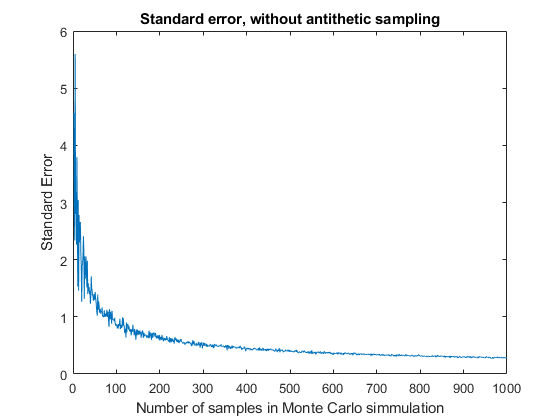
\includegraphics[width=1.1\textwidth]{StandardError.png}
        \caption{Standard Error without Antithetic Sampling}
    \end{minipage}
    \begin{minipage}{0.4\textwidth}
        \centering
        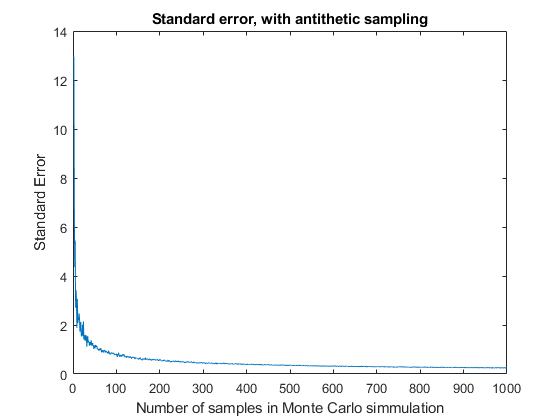
\includegraphics[width=1.1\textwidth]{StandardErrorAT.png}
        \caption{Standard Error with Antithetic Sampling}
    \end{minipage}
\end{figure}

We can see from the standard error graphs that both errors tend to 0 as the number of simmulations increases, 
although we can see that the line in the antithetic sampling figure is much thinner, due to the overall reduction 
in variance. \\

\subsection{Performance}
Including antithetic sampling in the Monte-Carlo simmulation greatly increases. The below table shows how the 
time to run changes with increasing number of simmulations both using and not using antithetic sampling.

\begin{table}[h]
\centering
\begin{tabular}{c c c c}
    Nmc & Non-Antithetic Time (s)& Antithetic Time (s) & Improved Antithetic \\
    100 & 0.0454 & 0.0691 & 0.0397 \\
    1000 & 0.3588 & 0.7000 & 0.3777 \\
    10000 & 3.6219 & 7.002 & 3.9213 \\
    100000 & 35.7083 & 71.5724 & 39.3678 
\end{tabular}
\label{MCTable}
\end{table}

We can see that although both increase exponentially, the version using antithetic sampling ends up roughly 
doubling the time taken by not using it. This is because we are calculating double the amount of samples, just with 
opposite coefficient on the drift term. So in order to increase performance, it was decided that instead of 
calculating $(r-\delta-\frac{\sigma^2}{2})(t_{i+1}-t_i)$ and $\sigma\sqrt{t_{i+1}-t_i}$ twice, we can calculate them at 
the start of the for-loop and call that value when it is needed. It can be seen in the final column of Table~\ref{MCTable}
that doing this cuts the time down by again around a half, so we get the reduced variance and increased performance.

\end{document}